\section{Design}\insertloftspace
\setcounter{figure}{0}\setcounter{table}{0}

\subsection{Brainstorming}

\subsection{Onshape}
\subsubsection{Presentation}

To model our robot, we used the software Onshape \cite{Onshape}. It is a computer-aided design software system, delivered over the Internet via a software as a service model. This software offers many advantages : 
\begin{itemize}[noitemsep]
    \item collaborative
    \item quick to learn
    \item online
\end{itemize}

The last one may limit its use because it requires an internet connection.

\subsubsection{Rules}

Rules to standardize our work have also been established from the beginning. As we will see in the following parts, it is necessary to respect them in order to be able to exploit these documents with other software.
\begin{itemize}
    \item Name all parts with a specific name: it is the ID of the part and it has to be unique
    \item One subassembly by articulation: a subassembly contains all the parts of an articulation that have a fixed join between them
    \item One main assembly containing the motor links: the main assembly contains only the join that you want to see at the end. Usually, it is the dynamic join but it can be fixed to get a part separately.
    \item Assign material to each part: in Onshape, you precise the volumic mass, you need to pay attention in case you use PLA with a 3D printer. A part is never full at 100\% and you need to adapt the volumic mass to get the correct masS.
    \item Motor link in the main assembly needs to be named \textit{dof\_\less link\_name\bg}
    \item A relation between parent/child needs to be respected for every link: In Onshape, like all CAO software, there is a parent/child relation in every link. You really need to pay attention to this, it can be a source of many errors if you want to export your model. When you create a link, fixed or motorized, the first element you click on is the child. The second one is the father. You can then check the parent and the child as shown in the following image. It is therefore necessary to start from the origin to the end of the robot, respecting these relationships at the time of assembly.
\end{itemize}
\begin{figure}[H]
    \centering
    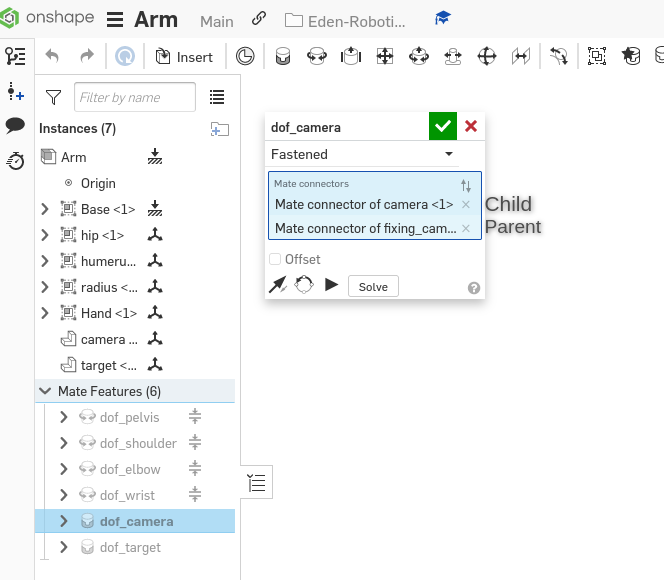
\includegraphics[width=0.5\textwidth]{Images/Section03/Parent_Child.png}
    \caption{Parent child principle}
    \label{fig:ParentChild}
\end{figure}

\subsection{Arm}

\subsection{Hand}

\subsection{Final version}